%%% TO DO %%%

\documentclass[12pt]{article}

\usepackage{ishn}
\usetikzlibrary{decorations.markings}
\usetikzlibrary{patterns}
\usetikzlibrary{patterns.meta}
\usetikzlibrary{arrows.meta}
\usepackage{siunitx}
\usepackage{etoolbox}
\usepackage{caption}
\usepackage{subcaption}

\makeindex[intoc]

\begin{document}
\robustify\dots
\sisetup{input-digits = 0123456789\dots}

\tikzset{middlearrow/.style={
        decoration={markings,
            mark= at position 0.5 with {\arrow{#1}} ,
        },
        postaction={decorate}
    }
}

\hypersetup{pageanchor=false}
\begin{titlepage}
	\begin{center}
		\vspace*{1em}
		\Huge
		\textbf{IB Fluid Dynamics}

		\vspace{1em}
		\large
		Ishan Nath, Lent 2023

		\vspace{1.5em}

		\Large

		Based on Lectures by Prof. John Lister

		\vspace{1em}

		\large
		\today
	\end{center}
	
\end{titlepage}
\hypersetup{pageanchor=true}

\tableofcontents

\newpage

\setcounter{section}{-1}

\section{Introduction}
\label{sec:introduction}

This course focuses on \emph{fluids}: we can think of these are liquids or gases, or more rigorously objects which are described well by the Navier-Stokes equations.

Studying fluids puts us in the realm of \emph{continuum mechanics}\index{continuum mechanics}, where materials are modelled with continuous mass; of course, we know in reality they are discrete particles. Areas of continuum mechanics include:
\begin{itemize}
	\item Fluid dynamics, concerned with liquids and gases.
	\item Solid mechanics, where we look at solids and their properties, and fracture mechanics.
	\item Other materials, such as complex fluid, soft matter, biomechanics, porous media, granular flow, and so on.
\end{itemize}

To obtain the continuum hypothesis, we average over the irrelevant molecular detail to get a continuous description in terms of \emph{fields}\index{fields}. Important examples are \emph{velocity} $\mathbf{u}(\mathbf{x},t)$, \emph{pressure} $p(\mathbf{x},t)$ and \emph{density} $\rho(\mathbf{x}, t)$

In this course, we take ideas in physics: mass, momentum, Newton's laws, vector calculus, and other methods and combine them to find properties of the fields and accompanying forces.

This course starts looking at \emph{kinematics}: properties of how fluids move, including velocities and trajectories. Then we delve into more serious \emph{dynamics}, involving forces and equations of motions.

For simplicity, we consider \emph{inviscid flow}. This gives a good approximation for water and air, apart from on small scales.

The obvious reason to study fluids is that fluids are everywhere: from our environment, in the oceans and atmosphere, to molecular biology; from aerosols to astrophysics.

\newpage

\section{Kinematics}
\label{sec:kinematics}

\subsection{Pathlines and Streamlines}
\label{sub:pathlines_and_streamlines}

There are two natural perspectives to view a fluid $\mathbf{u}(\mathbf{x}, t)$:
\begin{enumerate}
	\item A passive approach; as a stationary observer watching the flow go past (the \emph{Eulerian picture}).
	\item An active approach; as a moving observer, travelling along with (same part of) the flow (the \emph{Lagrangian picture}).
\end{enumerate}

Taking the passive approach, one way to visualise the fluid is using \emph{streamlines}. Streamlines\index{streamlines} are curves that are everywhere parallel to the flow at a given instant. These are given parametrically as
\[
	\mathbf{x} = \mathbf{x}(s;x_0, t_0), \text{ derived from } \frac{\diff \mathbf{x}}{\diff s} = \mathbf{u}(\mathbf{x}, t_0)
,\]
subject to initial condition $\mathbf{x} = \mathbf{x}_0$ at $s = 0$. These are similar to \emph{characteristics} (which we will see later). At a given time, the set of streamlines shows the direction of flow at that instant - it shows all particles, at a fixed time. For $\mathbf{u} = (1, t)$, we get the streamlines seen in figure~\ref{fig:streamlines_1_t}.

\begin{figure}[h]
\centering
\caption{Streamlines of $\mathbf{u} = (1, t)$ for different $t$}
\label{fig:streamlines_1_t}
\begin{subfigure}{0.5\textwidth}
	\centering
  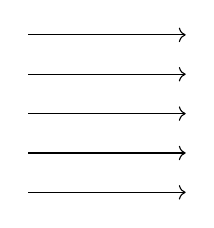
\begin{tikzpicture}
    \draw [->] (0,2) -- +(2,0);
    \draw [->] (0,1.5) -- +(2,0);
    \draw [->] (0,1) -- +(2,0);
    \draw [->] (0,0.5) -- +(2,0);
    \draw [->] (0,0) -- +(2,0);
  \end{tikzpicture}
  \caption{$t = 0$}
\end{subfigure}%
\begin{subfigure}{0.5\textwidth}
	\centering
	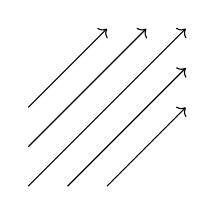
\begin{tikzpicture}
		\draw [->] (0,1) -- +(1,1);
		\draw [->] (0,0.5) -- +(1.5,1.5);
		\draw [->] (0,0) -- +(2,2);
		\draw [->] (0.5,0) -- +(1.5,1.5);
		\draw [->] (1,0) -- +(1,1);
	\end{tikzpicture}
	\caption{$t = 1$}
\end{subfigure}
\end{figure}

In contrast, a \emph{pathline}\index{pathline} is when we look at the trajectory of a fluid `particle' (which we can think of as a very small part of the fluid). The pathline $\mathbf{x} = \mathbf{x}(t; \mathbf{x}_0)$ of the particle that starts at $\mathbf{x}_0$ at $t = 0$ is found from
\[
\frac{\diff \mathbf{x}}{\diff t} = \mathbf{u}(\mathbf{x}, t)
,\]
with initial conditions $\mathbf{x} = \mathbf{x}_0$ at $t = 0$. The set of pathlines give the flow of one particle, at all times. The pathline of $\mathbf{u} = (1, t)$ is graphed in figure~\ref{fig:pathlines_1_t}.

\begin{figure}[h]
	\centering
	\caption{Pathlines of $\mathbf{u} = (1,t)$ for three initial points}
	\label{fig:pathlines_1_t}
	\begin{tikzpicture}
		\begin{axis}
			[
			xmin = 0,
			xmax = 3.1,
			ymin = 0,
			ymax = 1,
			axis lines = none
			]
		\addplot [domain = 0:1, smooth, ->] {x*x};
		\addplot [mark = *] coordinates {(0,0)};
		\addplot [domain = 1:2, smooth, ->] {(x-1) * (x-1)};
		\addplot [mark = *] coordinates {(1,0)};
		\addplot [domain = 2:3, smooth, ->] {(x-2) * (x-2)};
		\addplot [mark = *] coordinates {(2,0)};
		\end{axis}
	\end{tikzpicture}
\end{figure}

We can consider many particles, such as all $\mathbf{x}_0$ in a given region, to see how the shape and position of a dyed patch of fluid evolves. This is useful for thinking about transport and mixing problems.

For \emph{steady-state flows}\index{steady-state flows}, streamlines and pathlines are the same.

\subsection{The Material Derivative}
\label{sub:the_material_derivative}

Both streamlines and pathlines are taken from the Eulerian picture: we are sitting outside and watching the fluid go by. Things are different if we are drifting with the fluid.

In particular, for a field $F(\mathbf{x},t)$, which may be density or velocity or something else we want to know, we can measure it with respect to some fixed position. However, if we are moving along with the fluid, then this field is changing: we can parametrize it as $F(\mathbf{x}(t), t)$. We can calculate
\begin{align*}
	\delta F &= F(\mathbf{x} + \delta \mathbf{x}, t + \delta t) - F(\mathbf{x}, t) \\
		 &= \delta \mathbf{x} \cdot \nabla F + \delta t \frac{\partial F}{\partial t} + \mathcal{O}(\delta^2),
\end{align*}
and we know $\delta \mathbf{x} = \mathbf{u}(\mathbf{x},t) \delta t + \mathcal{O}(\delta^2)$, so these equations simplify to
\[
\frac{DF}{Dt} = \frac{\partial F}{\partial t} + \mathbf{u} \cdot \nabla F
,\]
where we use new notation for the total time derivative. The additional $\mathbf{u} \cdot \nabla F$ corresponds to the movement due to the fluid. This is called the \emph{material derivative}\index{material derivative}, as it describes the rate of change of a field, when moving through a fluid (or material).

\subsection{Conservation of Mass}
\label{sub:conservation_of_mass}

Consider a (rigid) tube with constant cross-section, with fluid coming in with speed $\mathbf{u} = 2$, and exiting with speed $\mathbf{u} = 1$.

For a fluid such as air, this could be conceivably possible: the air could be compressed in the tube.

However, with water this would be impossible, as the density of water $\rho_{\rm{water}}$ is relatively constant. Hence a difference in velocities means that mass is being destroyed.

This suggests that there must be a relationship between $\rho(\mathbf{x},t)$ and $\mathbf{u}(\mathbf{x},t)$ such that mass is never created or destroyed, so we go looking for such a relationship.

Consider an arbitrary volume $V$, fixed in space and bounded by a surface $\partial V$ with outwards normal $\mathbf{n}$. Then the mass in $V$, which is
\[
M = \int_{V} \rho \diff V
,\]
can only change if mass flows in or out at the surface $\partial V$. The amount of mass that escapes an area $A$ over time $t$ is $\rho \mathbf{u} \cdot \mathbf{n} \delta A \delta t$. We can think of $\rho \mathbf{u}$ as the \emph{mass flux}\index{mass flux}. Integrating over $V$,
\begin{align*}
	\frac{\diff}{\diff t} \int_{V} \rho \diff V &= - \int_{S} \rho \mathbf{u} \cdot \diff \mathbf{S}, \\
	\iff \int_{V} \frac{\partial p}{\partial t} \diff V &= - \int_{V} \nabla \cdot (\rho \mathbf{u}) \diff V,
\end{align*}
where we have used the divergence theorem. Since this holds for all volumes $V$, we must have
\[
\frac{\partial \rho}{\partial t} + \nabla \cdot (\rho \mathbf{u}) = 0
.\]
Using $\nabla \cdot (\rho \mathbf{u}) = \mathbf{u} \cdot \nabla \rho + \rho \nabla \cdot \mathbf{u}$, we can rewrite this as
\[
\frac{D \rho}{Dt} + \rho \nabla \cdot \mathbf{u} = 0
.\]
Physically, this means that if a fluid is flowing away from a point, the density should decrease, and vice versa.

If a fluid is \emph{incompressible}\index{incompressible}, then the density of the fluid is constant, so $\dot \rho = \nabla \rho = 0$. Hence the velocity must satisfy
\[
\nabla \cdot \mathbf{u} = 0
\]
for incompressible flow. In this course, we make the assumption that density is constant and uniform. This assumption is good when the speed of the fluid is much less than the speed of sound, which is around \qty{330}{\metre\per\second} in air, and \qty{1500}{\metre\per\second} in water.

\subsection{Kinematic Boundary Condition}
\label{sub:kinematic_boundary_condition}

Suppose that the material boundary of a body of fluid has velocity $\mathbf{U}(\mathbf{x},t)$. Then at a point $\mathbf{x}$ on the boundary of the fluid, the velocity relative to the moving boundary is $\mathbf{u}(\mathbf{x}, t) - \mathbf{U}(\mathbf{x}, t)$.

The condition that there is no mass flux across the boundary can be written as $\rho (\mathbf{u} - \mathbf{U}) \cdot \mathbf{n} \, \delta A \delta t=  0$, or
\[
\mathbf{n} \cdot \mathbf{u} = \mathbf{n} \cdot \mathbf{U}
.\]

\begin{exbox}
	\begin{enumerate}
		\item For a stationary rigid boundary, $\mathbf{U} = 0$, so we must have $\mathbf{u} \cdot \mathbf{n} = 0$.
		\item Water waves have an air-water interface $z = \eta(x, y, t)$. We can think of the water surface as a contour of the function $F(x, y, z, t) = z - \eta(x, y, t)$.

			Then the normal $\mathbf{n}$ will be parallel to $\nabla F = (-\eta_x, \eta_y, 1)$. Since $\mathbf{U} = (0, 0, \eta_t)$, if we take $\mathbf{u} = (u, v, w)$, the boundary flux condition implies
			\[
			- u \eta_x - v \eta_y + w = \eta_t
			.\]
			This is equivalent to
			\[
			\frac{D}{Dt}(z - \eta) = 0
			,\]
			which means that particles on the surface of the wave will stay on the surface.
	\end{enumerate}
\end{exbox}

\begin{figure}[h]
	\centering
	\caption{Surface of Water}
	\label{fig:water_surface}
	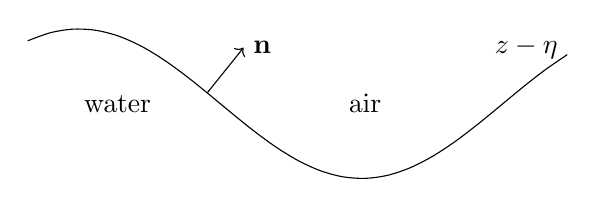
\begin{tikzpicture}
		\begin{axis}
			[
			xmin = 1,
			xmax = 7,
			ymin = -1,
			ymax = 1,
			axis lines = none
			]
			\addplot [smooth, domain = 1:7] {sin(deg(x))/3};
			\draw [->] (3,0.05) -- (3.4,0.25);
			\node [right] at (3.4, 0.25) {$\mathbf{n}$};
			\node at (4.75,0) {air};
			\node at (2,0) {water};
			\node [left] at (7, 0.25) {$z - \eta$};
		\end{axis}
	\end{tikzpicture}
\end{figure}

\subsection{Stream Function for 2D Incompressible Flow}
\label{sub:stream_function_for_2d_incompressible_flow}

Recall that a fluid is incompressible if $\nabla \cdot \mathbf{u} = 0$. However, this is equivalent to $\mathbf{u} = \nabla \times \mathbf{A}$ for some potential $\mathbf{A}$.

For two dimensional flows $\mathbf{u} = (u(x,y),v(x,y),0)$, we can take
\[
\mathbf{A} = (0, 0, \psi(x, y)) \implies \mathbf{u} = \biggl( \frac{\partial \psi}{\partial y}, - \frac{\partial \psi}{\partial x}, 0 \biggr)
.\]
Indeed, this implies
\[
\frac{\partial u}{\partial x} + \frac{\partial v}{\partial y} = 0
,\] 
so $\mathbf{u}$ is divergence-free, as expected. We say that $\psi(x, y)$ is the \emph{stream function}\index{stream function}.

The stream function satisfies the following properties:
\begin{enumerate}[(i)]
	\item The streamlines are given by $\psi = C$ (so $\mathbf{u}$ is parallel to the contours of $\psi$).
	\item $|\mathbf{u}| = |\nabla \psi|$, so the flow is faster where the streamlines are closer together.
	\item The volume that is crossing the line from $\mathbf{x}_0$ to $\mathbf{x}_1$ is
		\[
		\int_{\mathbf{x}_0}^{\mathbf{x}_1} \mathbf{u} \cdot \mathbf{n} \diff l = \psi(\mathbf{x}_1) - \psi(\mathbf{x}_0)
		.\]
	\item $\psi$ is constant on a stationary rigid boundary.
\end{enumerate}

\begin{exbox}
	Take $\mathbf{u} = (y, x)$. Since $\nabla \cdot \mathbf{u} = 0$, a stream function exists. Integrating the above equations,
	\begin{align*}
		\frac{\partial \phi}{\partial y} = y &\implies \psi = \frac{1}{2} y^2 + f(x), \\
		-\frac{\partial \psi}{\partial x} = x &\implies f(x) = -\frac{1}{2}x^2.
	\end{align*}
	Hence the streamlines are
	\[
		y^2 - x^2 = C
	.\]
\end{exbox}

In polar coordinates, we have $\mathbf{u} = (u_r(r, \theta), u_\theta(r, \theta), 0)$. If $\mathbf{A} = (0, 0, \psi(r, \theta))$, then
\[
\mathbf{u} = \nabla \times \mathbf{A} = \biggl( \frac{1}{r} \frac{\partial \psi}{\partial \theta}, - \frac{\partial \psi}{\partial r}, 0 \biggr)
.\]
We can verify that
\[
\nabla \cdot \mathbf{u} = \frac{1}{r} \frac{\partial}{\partial r} (r u_r) + \frac{1}{r} \frac{\partial u_{\theta}}{\partial \theta} = 0
.\]

Axisymmetric flow in spherical polar coordinates has
\[
u_{\phi} = \frac{\partial}{\partial \phi} = 0
.\]
If we have $\nabla \cdot \mathbf{u} = 0$, and we take
\[
\mathbf{A} = \biggl( 0, 0, \frac{\Psi(r, \theta)}{r \sin \theta} \biggr)
,\]
then
\[
\mathbf{u} = \biggl( \frac{1}{r^2 \sin \theta} \frac{\partial \Psi}{\partial \theta}, - \frac{1}{r \sin \theta} \frac{\partial \Psi}{\partial r}, 0 \biggr)
\]
is parallel to the contours of $\Psi$. Hence the contours of the Stokes stream $\Psi(r, \theta)$ form the stream tubes.

\newpage

\section{Dynamics of Inviscid Flow}
\label{sec:dynamics_of_inviscid_flow}

\subsection{Surface and Volume Forces}
\label{sub:surface_and_volume_forces}

There are two types of force which act on a fluid:
\begin{enumerate}[(i)]
	\item Those proportional to the volume, like gravity.
	\item Those proportional to the surface area, like pressure or \emph{viscous stress}, which is the friction between moving fluid and moving material, whether a boundary or another fluid.
\end{enumerate}
We look at these individually.

\begin{enumerate}[(i)]
	\item For \emph{volume} or \emph{body forces}\index{volume force}\index{body force}, we denote the force on a small volume element as $\mathbf{f}(\mathbf{x},t)\, \delta V$. Often, $\mathbf{f}$ is \emph{conservative}with potential energy per unit volume $\chi$, and hence $\mathbf{f} = - \nabla \chi$.

		The most common case for us is gravity; here $\mathbf{f} \, \delta V = \rho \mathbf{g} \, \delta V$, with $\chi = \rho g z$, where $\mathbf{g} = (0, 0, g)$.
	\item For a \emph{surface force}\index{surface force}, we consider a small element of area $\mathbf{n} \, \delta A$.

		Denote the surface force exerted by the outside on the inside by $\bm{\tau}(\mathbf{x}, t ; \mathbf{n}) \, \delta A$, where $\bm{\tau}$ is the \emph{stress}\index{stress} acting on the area element. Note that the stress $\bm{\tau}$ depends on the orientation $\mathbf{n}$.

		By Newton's third law, the surface force exerted by the inside on the outside is
		\[
		- \bm{\tau}(\mathbf{x}, t;\mathbf{n}) = \bm{\tau}(\mathbf{x}, t; \mathbf{n})
		.\]
		We defer discussion of viscous stresses to chapter 3. In fact, in many phenomena the viscous stresses are negligible and the fluid behaves as if it is \emph{inviscid}\index{inviscid} (frictionless).
\end{enumerate}


\begin{figure}[h]
	\centering
	\caption{Surface force on a small area $\delta A$}
	\label{fig:surface_force}
	\begin{tikzpicture}
		\draw (0,0) circle [x radius = 1,y radius = 2];
		\draw [->, thick] (0,0) -- +(2,0);
		\draw [->, thick, red] (-1,0) -- +(-1.5,0);
		\node at (-2,-1) {$\bm{\tau} = - p \mathbf{n}$};
		\node at (3, 1) {outside};
		\node at (-3, 1) {inside};
		\node [right] at (2,0) {$\mathbf{n}\, \delta A$};
	\end{tikzpicture}
\end{figure}

For inviscid fluids, the stress $\bm{\tau}$ acting across $\mathbf{n} \, \delta A$ has no tangential component, and has magnitude independent of the orientation:
\[
\bm{\tau}(\mathbf{x},t;\mathbf{n}) = - p(\mathbf{x},t)\mathbf{n}
,\]
where $p$ is the pressure. Note the sign: the outside pushes on the inside in the direction $- \mathbf{n}$.

\subsection{The Euler Momentum Equation}
\label{sub:the_euler_momentum_equation}

Consider an arbitrary volume $V$, fixed in space, bounded by surface $\partial V$ with an outward normal $\mathbf{n}$.

The momentum $\int_{V} p \mathbf{u}\diff V$ inside $V$ can change due to:
\begin{enumerate}[(i)]
	\item Flow of momentum across the boundary $\partial V$,
	\item Volume/body forces,
	\item Surface Forces.
\end{enumerate}

Recall the volume out across $\delta A$ in time $\delta t$ is $\mathbf{n} \, \delta A \cdot \mathbf{u} \, \delta t$, and the momentum out is $\rho \mathbf{u} (\mathbf{u} \cdot \mathbf{n} \, \delta A \delta t)$. Hence,
\[
\frac{\diff}{\diff t} \int_{V} \rho \mathbf{u} \diff V = - \int_{\partial V} \rho \mathbf{u}(\mathbf{u} \cdot \mathbf{n}) \diff A + \int_{\partial V} (- p \mathbf{n}) \diff A + \int_{V} \mathbf{f} \diff V
.\]

Here $\rho u_i u_j$ is the momentum flux, a second order tensor. We can rewrite this in terms of components as
\begin{align*}
	\frac{\diff}{\diff t} \int_{V} \rho u_i \diff V &= - \int_{\partial V} (\rho u_i u_j) n_j \diff A - \int_{\partial V} p n_i \diff A + \int_{V} f_i \diff V \\
	\iff \int_{V} \frac{\partial}{\partial t} (\rho u_i) \diff V &= - \int_{V} \frac{\partial}{\partial x_j} (\rho u_i u_j) \diff V - \int_{V} \frac{\partial f}{\partial x_i} \diff V + \int_{V} f_i \diff V.
\end{align*}
Since $V$ is arbitrary, we obtain
\[
\frac{\partial}{\partial t}(\rho u_i) + \frac{\partial}{\partial x_j}(\rho u_i u_h) = - \frac{\partial f}{\partial x_i} + f_i
.\]
The left hand side can be expanded as
\begin{align*}
	LHS &= u_i \biggl( \frac{\partial \rho}{\partial t} + \frac{\partial}{\partial x_j} (\rho u_j)\biggr) + \rho \frac{\partial u_i}{\partial t} + \rho u_j \frac{\partial u_i}{\partial x_j} \\
	    &= \rho \biggl(\frac{\partial}{\partial t} + \mathbf{u} \cdot \nabla\biggr) u_i,
\end{align*}
due to mass conservation. What we are left with is the material derivative, so we get
\[
\rho \frac{D \mathbf{u}}{D t} = - \nabla p + \mathbf{f}
.\]
This is the \emph{Euler momentum equation}\index{Euler momentum equation}.

The Euler momentum equation also has a dynamic boundary condition, which says that the stress $\bm{\tau}$ exerted on the fluid by the boundary is $-p \mathbf{n}$.

\begin{exbox}
	Consider a bent hose pipe with steady uniform flow $U$ in and out, with constant cross-sectional area $A$. We neglect gravity (so $\mathbf{f} = 0$).

	From the momentum integral equation, the momentum inside the volume is unchanging, and $\mathbf{f} = 0$, so this simplifies to
	\[
		\int_{\rm{walls}} [\rho \mathbf{u}(\mathbf{u} \cdot \mathbf{n}) + p \mathbf{n}] \diff A + \int_{\rm{ends}} [\rho \mathbf{u} (\mathbf{u} \cdot \mathbf{n}) + p \mathbf{n}] \diff A = 0
	.\]
	We know that
	\[
		\int_{\rm{walls}} [\rho \mathbf{u}(\mathbf{u} \cdot \mathbf{n}) + p \mathbf{n}] \diff A = \int_{\rm{walls}} p \mathbf{n} \diff A
	,\]
	as the walls are rigid, so $\mathbf{u} \cdot \mathbf{n} = 0$. This is simply the force by the fluid on the pipe. Moreover, on the ends
	\[
		\int_{\rm{ends}}[\rho \mathbf{u}(\mathbf{u} \cdot \mathbf{n}) + p \mathbf{n}] \diff A = A [p_1 \mathbf{n}_1 + \rho(-U \mathbf{n}_1)(-U) + p_2 \mathbf{n}_2 + \rho(U \mathbf{n}_2)U]
	.\]
	In fact we get $p_1 = p_2$. Hence the force on the pipe is
	\[
	-A (p + \rho U^2)(\mathbf{n}_1 + \mathbf{n}_2)
	.\]
	The $\rho U^2$ contribution comes from the change in momentum flux: the fluid in changes direction.
\end{exbox}

\subsection{Bernoulli's Equation for Steady Flow with Potential Forces}
\label{sub:bernoullis_equation_for_steady_flow_with_potential_forces}

Recall the Euler equation

\[
\rho \biggl( \frac{\partial \mathbf{u}}{\partial t} + (\mathbf{u} \cdot \nabla) \mathbf{u} \biggr) = - \nabla p + \mathbf{f}
.\]
For steady flows, the change in time will be 0. Moreover, we can rewrite the potential forces as $\mathbf{f} = - \nabla \chi$. Using the vector identity
\[
\mathbf{u} \times (\nabla \times \mathbf{u}) = \nabla \biggl( \frac{1}{2} u^2 \biggr) - (\mathbf{u} \cdot \nabla)\mathbf{u}
,\]
where $u = |\mathbf{u}|$, we can introduce the \emph{vorticity}\index{vorticity}
\[
\mathbf{w} = \nabla \times \mathbf{u}
\]
to reduce the Euler equation to
\begin{align*}
	\rho \biggl( 0 + \nabla \biggl( \frac{1}{2} u^2 \biggr) - \mathbf{u} \times \mathbf{w} \biggr) &= - \nabla p - \nabla \chi \\
	\iff \nabla \biggl( \frac{1}{2} \rho u^2 + p + \chi \biggr) &= \rho \mathbf{u} \times \mathbf{w} \\
	\iff \mathbf{u} \cdot \nabla \biggl( \frac{1}{2} \rho u^2 + p + \chi \biggr) &= 0.
\end{align*}
Hence
\[
H = \frac{1}{2} \rho u^2 + p + \chi
\]
is constant along streamlines. This is \emph{Bernoulli's equation}\index{Bernoulli's equation}.

Since $H$ is constant, $p$ is low where $u$ is high, and vice versa.


\begin{figure}[h]
	\centering%do later
	\caption{Water Container}
	\label{fig:container}
	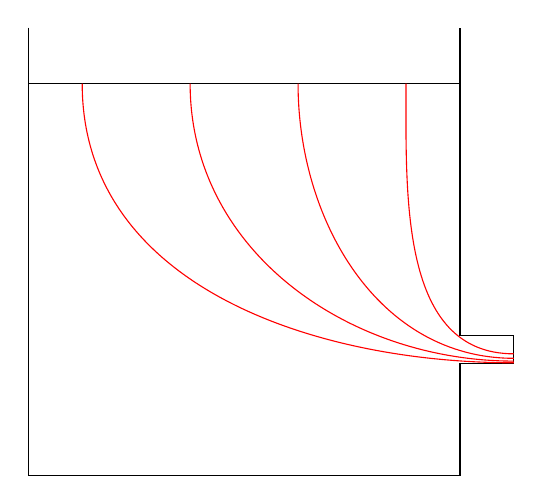
\begin{tikzpicture}
		\begin{axis}
			[
			xmin = -5,
			xmax = 5,
			ymin = 0,
			ymax = 4,
			axis lines = none
			]
			\draw [-] (-4,4) -- (-4,0) -- (4,0) -- (4,1) -- (5,1) -- (5,1.25) -- (4,1.25) -- (4,4);
			\draw [-] (-4,3.5) -- (4,3.5);
			\draw [red] (3,3.5) to[out = -90,in=180] (5,1.09);
			\draw [red] (1,3.5) to[out = -90, in = 180] (5,1.05);
			\draw [red] (-1,3.5) to[out = -90, in = 180] (5,1.025);
			\draw [red] (-3,3.5) to[out = -90, in = 180] (5,1.01);
		\end{axis}
	\end{tikzpicture}
\end{figure}

At the surface of the water, we have a large area, with $u \approx 0$, $\chi = 0$ and $p = p_a$.

At the small exit tube, $\chi = - \rho g h$, $p = p_a$ (as the water is next to the air), and so by Bernoulli, $u = \sqrt{2gh}$.

At a point in the water, $u \approx 0$, $\chi = - \rho g h$ and $p = p_a + \rho g h$.

\begin{figure}[h]
	\centering%do later
	\caption{Pitot Tube}
	\label{fig:pitot_tube}
	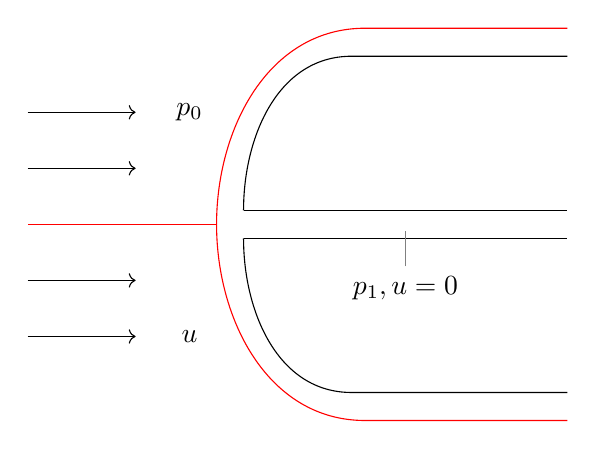
\begin{tikzpicture}
		\begin{axis}
			[
			xmin = -5,
			xmax = 5,
			ymin = 0,
			ymax = 4,
			axis lines = none
			]
			\draw [-] (-1, 2.125) -- (5, 2.125);
			\draw [-] (-1, 1.875) -- (5, 1.875);
			\draw [-] (-1, 2.125) to[out=90,in=180] (1, 3.5) to (5,3.5);
			\draw [-] (-1, 1.875) to[out=-90,in=180] (1, 0.5) to (5,0.5);
			\draw [red] (5,3.75) to (1.25,3.75) to[out=180,in=90] (-1.5, 2) to[out=-90,in=180] (1.25,0.25) to (5,0.25);
			\draw [red] (-1.5,2) -- (-5,2);
			\node [pin, anchor=north] at (2, 1.625) {$p_1, u = 0$};
			\node at (-2, 3) {$p_0$};
			\draw [->] (-5, 3) -- (-3, 3);
			\draw [->] (-5, 2.5) -- (-3, 2.5);
			\draw [->] (-5, 1.5) -- (-3, 1.5);
			\draw [->] (-5, 1) -- (-3, 1);
			\node at (-2, 1) {$u$};
		\end{axis}
	\end{tikzpicture}
\end{figure}

Using Bernoulli along the stagnation line,
\[
	\frac{1}{2} \rho_{\rm{air}} u^2 + p_0 = 0 + p_1 \implies u = \biggl[ \frac{2(p_1 - p_0)}{\rho_{\rm{air}}} \biggr]^{1/2}
.\]

\begin{figure}[h]
	\centering%do later
	\caption{Venturi Meter}
	\label{fig:venturi_meter}
	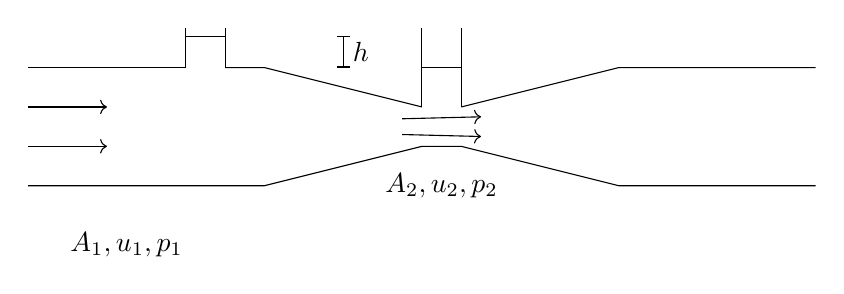
\begin{tikzpicture}
			\draw [-] (-5,3) -- (-3,3);
			\draw [-] (-2.5,3) -- (-2,3) -- (0,2.5);
			\draw [-] (0.5,2.5) -- (2.5,3) -- (5,3);
			\draw [-] (-5,1.5) -- (-2,1.5) -- (0,2) -- (0.5,2) -- (2.5,1.5) -- (5,1.5);
			\draw [-] (-3,3.5) -- (-3,3);
			\draw [-] (-2.5,3.5) -- (-2.5,3);
			\draw [-] (-3, 3.4) -- (-2.5,3.4);
			\draw [-] (0, 3) -- (0.5, 3);
			\draw [|-|] (-1, 3.4) -- (-1, 3);
			\node [right]at (-1, 3.2) {$h$};
			\draw [-] (0,3.5) -- (0, 2.5);
			\draw [-] (0.5,3.5) -- (0.5, 2.5);
			\draw [->] (-5,2) -- (-4, 2);
			\draw [->] (-5,2.5) -- (-4, 2.5);
			\draw [->] (-0.25,2.15) -- (0.75, 2.125);
			\draw [->] (-0.25,2.35) -- (0.75, 2.375);
			\node at (-3.75,0.75) {$A_1, u_1, p_1$};
			\node at (0.25,1.5) {$A_2, u_2, p_2$};
	\end{tikzpicture}
\end{figure}

Assume steady flow, so it is uniform across a cross section. This is alright for gentle variation of $A$. Due to mass conservation,
\[
A_1 u_1 = A_2 u_2 = Q
.\]
Due to Bernoulli,
\[
\frac{1}{2} \rho u_1^2 + p_1 = \frac{1}{2} \rho u_2^2 + p_2 \implies p_1 - p_2 = \frac{1}{2} \rho u_1^2 \biggl( \frac{A_1^2}{A_2^2} - 1 \biggr) > 0
.\]
We can measure $h$ to get $\rho gh = p_1 - p_2 = u_1$, so
\[
	Q = \sqrt{2 g h} \frac{A_1 A_2}{\sqrt{A_1^2 - A_1^2}}
.\]

We cannot use Bernoulli for a sudden enlargement of a pipe, as there will be complex unsteady flow with energy loss.

\begin{figure}[h]
	\centering%do later
	\caption{Large Change in Pipe}
	\label{fig:lcip}
	\begin{tikzpicture}
			\draw [-] (-5, 2.75) -- (-1, 2.75) -- (-1,4) -- (6,4);
			\draw [-] (-5, 1.25) -- (-1, 1.25) -- (-1,0) -- (6,0);
			\draw [red, ->] (-1, 2.75) -- (2, 2.75);
			\draw [red, ->] (-1, 1.25) -- (2, 1.25);
			\draw [red, ->] (3.5, 3) to[out=0, in=-45] (3.75,3.75);
			\draw [red, ->] (3.5, 1) to[out=0, in=45] (3.75,0.25);
			\node at (0.5, 2) {jet};
			\node at (0.5, 3.25) {still};
			\node at (0.5, 0.75) {still};
			\draw [->] (-5,1.5) -- (-3, 1.5);
			\draw [->] (-5,2) -- (-3, 2);
			\draw [->] (-5,2.5) -- (-3, 2.5);
			\node at (-2.5, 2.5) {$u_0$};
			\node at (-2.5, 2) {$p_0$};
			\node at (-2.5, 1.5) {$A_0$};
			\draw [->] (5,3) -- (6, 3);
			\draw [->] (5,2) -- (6, 2);
			\draw [->] (5,1) -- (6, 1);
			\node at (6.5, 3) {$u_1$};
			\node at (6.5, 2) {$p_1$};
			\node at (6.5, 1) {$A_1$};
	\end{tikzpicture}
\end{figure}

Assuming that $p_{\rm{jet}} = p_{\rm{still}}$, so there is no sideways acceleration, and $p_{\rm{jet}} = p_0$, applying the momentum integral equation to the box, with $\mathbf{f} = 0$, we get
\[
\frac{\diff}{\diff t} \Biggl( \int \rho \mathbf{u} \diff V \Biggr) \approx 0
.\]

\begin{figure}[h]
	\centering%do later
	\caption{Momentum Integral for Large Change}
	\label{fig:milc}
	\begin{tikzpicture}
			\draw [-] (-5, 2.75) -- (-1, 2.75) -- (-1,4) -- (6,4);
			\draw [-] (-5, 1.25) -- (-1, 1.25) -- (-1,0) -- (6,0);
			\draw [dashed, red] (-0.75, 0.25) -- (6, 0.25) -- (6,3.75) -- (-0.75, 3.75) -- (-0.75, 0.25);
			\draw [->] (-0.75, 3.5) -- (-1.25, 3.5);
			\node at (-1.5, 3.5) {$\mathbf{n}$};
			\draw [->] (6, 3) -- (6.5,3);
			\node at (6.25,2.5) {$\mathbf{n}$};
	\end{tikzpicture}
\end{figure}

Then we can show that
\[
p_1 = p_0 + \rho u_1^2 \biggl( \frac{A_1}{A_0} - 1 \biggr) \biggl( \frac{A_1}{A_0} \biggr)
.\]

Now consider a water jet hitting an oblique wall. We will consider a two-dimensional case, where we neglect gravity. Assume the cross section of the incoming fluid is $a$, and has speed $U$, and the area going up is $a_2$, and going down is $a_1$.

\begin{figure}[h]
	\centering%do later
	\caption{Oblique Wall}
	\label{fig:oblique_wall}
	\begin{tikzpicture}
			\draw [-] (1, -3) -- (7, 1);
			\draw [-] (3.5,-0.5) -- (4.75,-0.5);
			\draw [-] (0, 0) to (3,0) to[out=0,in=-150] (6,1.25);
			\draw [-] (0, -1) to (2.5, -1)[out=0,in=30] to (0.5, -2.95);
			\node at (0, 0.5) {$u$};
			\node at (2, 0.5) {$p_a$};
			\draw [->] (5.9,0.6) -- (6.4, 0.95);
			\draw [->] (5.75,0.75) -- (6.25, 1.1);
			\draw [->] (2, -2.15) -- (1.5,-2.5);
			\node at (2,-2.75) {$a_1$};
			\node at (6.5, 1.25) {$a_2$};
			\draw [|-|] (0.5, -0.1) -- (0.5, -0.9);
			\node [right] at (0.5, -0.5) {$a$};
	\end{tikzpicture}
\end{figure}

At the contact point of the stream and the wall, there will be pressure $p > p_a$, implying there is a force.

Using Bernoulli on the surface streamline where $p = p_a$ is constant, then the speed is constant along the streamline. Hence far from the impact where flow is uniform and $p = p_a$, we have $u = U$, so by mass conservation, $aU = a_1U + a_2U$.

The momentum integral equation applied to this gives
\[
\frac{\diff}{\diff t} \int_{V} \rho \mathbf{u} \diff V = - \int_{\partial V} \rho \mathbf{u} (\mathbf{u} \cdot \mathbf{n}) + p \mathbf{n} \diff A + \int_{V} \mathbf{f} \diff V
.\]

The time derivative is 0, as the flow is steady, and we neglect gravity. Hence we get
\[
\int_{\partial V} \rho \mathbf{u} (\mathbf{u} \cdot \mathbf{n}) + p \mathbf{n} \diff A
.\]

Note that $p = p_a$ apart from near the impact, and $\mathbf{u} \cdot \mathbf{n} = 0$ apart from the ends. Hence, the component parallel to the plane going upwards is
\[
-\rho U^2 a \cos \beta + p U^2 a_2 - p U^2 a_1
,\]
which we can solve (using conservation of mass) to get
\[
a_2 = a \frac{1 + \cos \beta}{2}, \qquad a_1 = a \frac{1 - \cos \beta}{2}
.\]
The component perpendicular to the plane is
\[
\frac{1}{2} \rho U^2 a \sin \beta = \int_{\partial V} p \mathbf{n} \diff A = \int_{\partial V} (p - p_a)\mathbf{n} \diff A
,\]
which is the force on the wall.

\subsection{Hydrostatic Pressure and Archimedes Principle}
\label{sub:hydrostatic_pressure_and_archimedes_principle}

If $\mathbf{u} = 0$, then by Euler,
\[
0 = - \nabla p + \rho \mathbf{g} = - \nabla (p + \chi)
,\]
\[
	\implies p + \chi = \mathrm{constant} \implies p = p_0 - pgz
.\]
This is the \emph{hydrostatic pressure}\index{hydrostatic pressure}.

We can also calculate the pressure force on a submerged body with $\mathbf{u} = 0$, in a fluid with density $\rho_{f}$:
\begin{align*}
	\mathbf{F} = - \int p \mathbf{n} \diff A = - \int (p_0 - \rho g z) \mathbf{n} \diff A = - \int \nabla (p_0 - \rho g z) \diff V = \rho_{f} g \mathbf{\hat z} V.
\end{align*}

Hence \emph{Archimedes principle}\index{Archimedes principle} says the upthrust or buoyancy is the weight of the fluid displaced.

For $\mathbf{u} \neq 0$ and constant $\rho$ everywhere, we can write $p = p_0 - \rho g z + p'$, and get
\[
\rho \frac{D \mathbf{u}}{D t} = - \nabla p'
.\]
Here $p'$ is the \emph{dynamic}\index{dynamic pressure} or \emph{modified} pressure. This is the variation due to the motion after subtracting the hydrostatic balance.

We can ignore gravity if there are no density variations and no free surfaces. If there is a free surface between air and water, then since $\rho_{\rm{water}} \neq \rho_{\rm{air}}$, gravity has an effect, leading to waves.

\subsection{Vorticity}
\label{sub:vorticity}\index{vorticity}

Vorticity is defined by
\[
\bm{\omega} = \nabla \times \mathbf{u}
.\]
This is another way to talk about the angular momentum of the fluid.

\begin{exbox}

	\begin{enumerate}
		\item If $\mathbf{u} = \bm{\Omega} \times \mathbf{x}$, this is solid-body rotation, and gives $\bm{\omega} = 2 \bm{\Omega}$.
		\item If $\mathbf{u} = (0, \gamma_x, 0)$, this is a simple shear, and gives $\bm{\omega} = (0, 0, \gamma)$.
		\item If $\mathbf{u} = (0, \frac{\kappa}{2 \pi r}, 0)$ in cylindrical polars, this is known as a line vortex with $\bm{\omega} = \mathbf{0}$ except at $r = 0$. Indeed, doing the line integral around the singularity gives
			\[
			\oint_{r = a} \mathbf{u} \cdot \diff \mathbf{l} = \int_{0}^{2 \pi} \frac{R}{2 \pi r} r \diff \theta = R
			,\]
			but using Stokes' theorem gives
			\[
			\oint_{r = a} \mathbf{u} \cdot \diff \mathbf{l} = \int_{r < a} \bm{w} \cdot \mathbf{\hat z} \diff A
			,\]
			hence we get $\bm{\omega} = (0, 0, \kappa \delta(r))$.
	\end{enumerate}

\end{exbox}

\subsubsection{Interpretation of Vorticity}
\label{subsub:interpretation_of_vorticity}

Consider a material line element $\delta \mathbf{l}$, moving with the fluid.

\begin{figure}[h]
	\centering%do later
	\caption{Line Element}
	\label{fig:line_element}
	\begin{tikzpicture}
		\draw [middlearrow={>}, blue] (0,0) -- (0,2);
		\draw [middlearrow={>}, red] (0,0) -- (3,-1);
		\draw [middlearrow={>}, blue] (3,-1) -- (4,3);
		\draw [middlearrow={>}, red] (0,2) -- (4,3);
		\node[below] at (0,0) {\small $\mathbf{x}$};
		\node[left] at (0,1) {\small $\delta \mathbf{l}(t)$};
		\node[below] at (3,-1) {\small $\mathbf{x}+\mathbf{u}(\mathbf{x},t)\delta t$};
		\node[right] at (3.5,1) {\small $\delta \mathbf{l}(t + \delta t)$};
		\node[above] at (0,2) {\small $\mathbf{x} + \delta \mathbf{l}$};
		\node[right] at (4,3) {\small $\mathbf{x} + \delta \mathbf{l} + \mathbf{u}(\mathbf{x} + \delta \mathbf{l}, t) \delta t$};
	\end{tikzpicture}
\end{figure}

Then $\delta \mathbf{l} \to \delta \mathbf{l} + (\delta \mathbf{l} \cdot \nabla) \mathbf{u} \delta t$, or
\[
\frac{\diff}{\diff t} \delta \mathbf{l} = (\delta \mathbf{l} \cdot \nabla) \mathbf{u}
.\]
Hence the tensor $\partial u_i/\partial x_j$ determines the rate of change of $\delta \mathbf{l}$. We can write
\[
\frac{\partial u_i}{\partial x_j} = \frac{1}{2} \biggl( \frac{\partial u_i}{\partial x_j} + \frac{\partial u_j}{\partial x_i} \biggr) + \frac{1}{2} \biggl( \frac{\partial u_i}{\partial x_j} - \frac{\partial u_j}{\partial x_i} \biggr) = e_{ij} + \frac{1}{2} \eps_{jik} \omega_{k}
.\]


The local rotation of line elements due to the second term is
\[
\frac{1}{2} \eps_{jik}\omega_k \delta l_j = \frac{1}{2} (\bm{w} \times \delta \mathbf{l})
.\]
The local motion due to the first term is called the \emph{strain rate}, which gives zero angular velocity averaged over all orientation $\delta \mathbf{l}$. $\mathbf{e}$ is symmetric and traceless when $\nabla \cdot \mathbf{u} = 0$.

Note that $\frac{1}{2} \bm{\omega}$ gives the rate of rotation of blobs, not whether the blobs are going in circles.

\subsubsection{Vorticity Equation}
\label{subsub:vorticity_equation}

Start with the identity
\[
\rho \biggl( \frac{\partial \mathbf{u}}{\partial t} + (\mathbf{u} \cdot \nabla) \mathbf{u} \biggr) = - \nabla p + \mathbf{f}
.\]
Assuming that $\rho$ is constant and $\mathbf{f}$ is conservative, if we take the earlier vector identity
\[
	(\mathbf{u} \cdot \nabla) \mathbf{u} = \nabla \biggl( \frac{1}{2} u^2 \biggr) - \mathbf{u} \times \bm{\omega}
,\]
hence taking the curls
\[
\rho \biggl( \frac{\partial \bm{\omega}}{\partial t} - \nabla \times (\mathbf{u} \times \bm{\omega}  \biggr) = 0
.\]
The second vector equation gives
\[
\nabla \times (\mathbf{u} \times \bm{\omega}) = (\bm{\omega} \cdot \nabla) \mathbf{u} - \mathbf{u} \cdot \nabla \bm{\omega}
.\]
Hence we get
\[
\frac{D \bm{\omega}}{D t} = \frac{\partial \bm{\omega}}{\partial t} + (\mathbf{u} \cdot \nabla) \bm{\omega} = (\bm{\omega} \cdot \nabla) \mathbf{u}
.\]
Hence moving with the fluid, $\bm{\omega}$ changes if $\mathbf{u}$ changes in the direction of $\bm{\omega}$.

\subsubsection{Vorticity Stretching}
\label{subsub:vorticity_stretching}

Compare the equations
\[
\frac{\diff}{\diff t} \delta \mathbf{l} = (\delta \mathbf{l} \cdot \nabla) \mathbf{u}, \qquad \frac{D \bm{\omega}}{D t} = (\bm{\omega} \cdot \nabla)\mathbf{u}
.\]
Moving with the fluid, $\bm{\omega}$ changes just like a material line element $\delta \mathbf{l}$ initially aligned with $\bm{\omega}$. In particular, if $\delta \mathbf{l}$ gets longer, then $\bm{\omega}$ gets bigger. This is just conservation of angular momentum.

For example, consider a uniformly rotating fluid cylinder. If over time the fluid stretches, then from mass conservation and angular momentum,
\begin{align*}
	a_1^2 \ell_1 &= a_2^2 \ell_2 & a_1^{6} \ell_1 \omega_1 &= a_2^{6} \ell_2 \omega_2,
\end{align*}
Rearranging, we get
\[
	\omega_2 = \omega_1 \frac{\ell_2}{\ell_1}
.\]
So $\bm{\omega}$ increases as fluid stretches in the direction of existing vorticity. This is called \emph{vortex stretching}\index{vortex stretching}, or the ballerina effect.

\begin{figure}[h]
	\centering
	\caption{Vortex Stretching}
	\label{fig:vortex_stretching}
	\begin{tikzpicture}
		\draw (2, -3) -- (2, 3);
		\draw (4, -3) -- (4, 3);
		\draw (3,3) circle (1 and 0.3);
		\draw (2,-3) arc (180:360:1 and 0.3);
		\draw (3,3) -- (3.5,3.258);
		\node[below] at (3.5, 3.203) {\small $a_2$};
		\draw (-4, -1.5) -- (-4, 1.5);
		\draw (0, -1.5) -- (0, 1.5);
		\draw (-2,1.5) circle (2 and 0.6);
		\draw (-4,-1.5) arc (180:360:2 and 0.6);
		\draw (-2,1.5) -- (-1,2.016);
		\node[below] at (-1,1.916) {\small $a_1$};
		\draw[|-|] (-4.2,-1.5) -- (-4.2,1.5);
		\node[left] at(-4.2,0) {\small $\ell_1$};
		\draw[|-|] (4.2,-3) -- (4.2,3);
		\node[right] at(4.2,0) {\small $\ell_2$};
		\draw[->] (0.5,0) -- (1.5,0);
		\draw[->] (-2,1.5) -- (-2,2.5);
		\draw[->] (3, 3) -- (3, 4);
		\draw[->] (-2, 1.9) + (120:0.4 and 0.12) arc (120:420:0.4 and 0.12);
		\node[above right] at (-2, 2) {\small $\omega_1$};
		\draw[->] (3, 3.6) + (120:0.4 and 0.12) arc (120:420:0.4 and 0.12);
		\node[above right] at (3, 3.6) {\small $\omega_2$};
	\end{tikzpicture}
\end{figure}

\begin{exbox}
	If we have
	\[
	\mathbf{u} = \biggl( - \frac{1}{2} \beta_x, - \frac{1}{2} \beta_y, \beta_z \biggr) + \Omega(t)(y, -x, 0)
	,\]
	then we can check
	\[
	\bm{\omega} = (0, 0, 2 \Omega)
	.\]
	Hence from
	\[
	\frac{\partial \bm{\omega}}{\partial t} + (\mathbf{u} \cdot \nabla) \bm{\omega} = (\bm{\omega} \cdot \nabla)\mathbf{u}
	,\]
	looking at the $z$-component, we get
	\[
	2 \dot \Omega = \Omega \beta
	,\]
	or $\Omega \propto e^{\beta t}$.
\end{exbox}

\subsubsection{Circulation}
\label{subsub:circulation}

The \emph{circulation}\index{circulation} around a closed curve $\Gamma$ is defined by
\[
C(\Gamma) = \oint_{\Gamma} \mathbf{u} \cdot \diff \mathbf{l} = \int_{S} \bm{\omega} \cdot \diff \mathbf{S}
,\]
by Stokes' theorem. For example, a line vortex 
\[
\mathbf{u} = \biggl(0, \frac{\kappa}{2 \pi r}, 0 \biggr)
\]
has circulation $\kappa$ for any circle $r = a$.

One further result about circulation is Kelvin's circulation theorem.\index{Kelvin's circulation theorem} This says if $\Gamma(t)$ is a material curve, i.e. one that is moving with the fluid, then
\[
	\frac{\diff}{\diff t}[C(\Gamma)] = \oint \biggl( \frac{D \mathbf{u}}{Dt} \diff \mathbf{l} + \mathbf{u} \cdot \frac{\diff}{\diff t} \delta \mathbf{l} \biggr) = 0
.\]
This can be seen by rewriting $Du/Dt$ using the Euler momentum equation, and noticing $\diff \delta\mathbf{l}/\diff t = (\mathbf{u} \cdot \nabla) \delta \mathbf{l}$:
\begin{align*}
	\frac{\diff}{\diff t} \oint_{\Gamma} \mathbf{u} \cdot \diff \mathbf{l} &= \oint_{\Gamma} \frac{Du}{Dt} \cdot \delta \mathbf{l} + \mathbf{u} \cdot \frac{\diff}{\diff t} \delta \mathbf{l} \\
									   &= \oint_{\Gamma} - \nabla \biggl( \frac{p + \chi}{p} \biggr) \cdot \diff \mathbf{l} + \mathbf{u} \cdot (\delta \mathbf{l} \cdot \nabla) \mathbf{u} \\
									   &= \biggl[ - \frac{p + \chi}{p} + \frac{1}{2} u^2 \biggr]_{\Gamma} = 0.
\end{align*}


Hence above, $C = \pi a^2(2 \Omega)$ is constant.

\newpage

\section{Introduction to Viscous Flow}
\label{sec:introduction_to_viscous_flow}

Chapter 2 was all about \emph{inviscid} flow.

We neglected friction (viscous stresses) between layers of fluid or boundaries. Inviscid fluid exerted only a normal stress $-p \mathbf{n}$. The forces $- \nabla p + \mathbf{f}$ were balanced by $\rho \cdot D\mathbf{u}/Dt$. If $\mathbf{f} = - \nabla \chi$, we also found that the energy and angular momentum are conserved.

With viscous flow, we will find:

Velocity gradients give rise to viscous stresses (friction), and fluids also exert tangential (shear) stresses on boundaries. In the momentum equation, we will have another term, and there is dissipation of energy and diffusion of vorticity.

\subsection{Plane Couette Flow and Viscosity}
\label{sub:plane_couette_flow_and_viscosity}

\begin{figure}[h]
	\centering
	\caption{Couette Flow}
	\label{fig:couette_flow}
	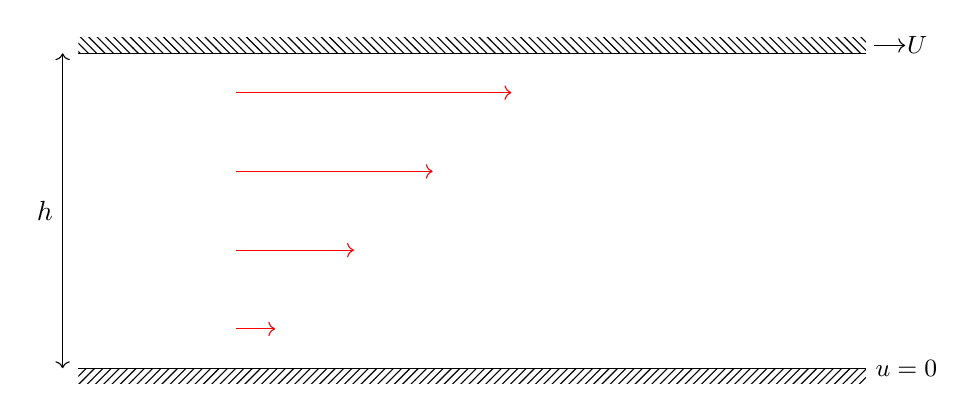
\begin{tikzpicture}
		\draw (-5, -2) -- (5, -2);
		\draw (-5, 2) -- (5, 2);
		\draw[red, ->] (-3, -1.5) -- (-2.5, -1.5);
		\draw[red, ->] (-3, -0.5) -- (-1.5, -0.5);
		\draw[red, ->] (-3, 0.5) -- (-0.5, 0.5);
		\draw[red, ->] (-3, 1.5) -- (0.5, 1.5);
		\node[right] at (5,-2) {\small $u=0$};
		\draw[->] (5.1,2.1) -- (5.5,2.1);
		\node[right] at (5.4,2.1) {\small $U$};
		\draw[<->] (-5.2, -2) -- (-5.2, 2);
		\node[left] at (-5.2, 0) {$h$};
		\fill[pattern = north west lines] (-5,2) rectangle +(10,0.2);
		\fill[pattern = north east lines] (-5,-2) rectangle +(10,-0.2);
	\end{tikzpicture}
\end{figure}

\emph{Couette flow}\index{Couette flow} is steady flow between parallel plates driven only by the motion of the top plate. We can find experimentally that for simple (Newtonian) fluids, that
\begin{enumerate}[(i)]
	\item Fluid velocity is $U$ on the top plate and $0$ on the bottom plate.
	\item Velocity varies linearly between these values.
	\item The tangential force per unit area $\tau_s$ required to move the top plate is proportional to $\frac{U}{h}$.
\end{enumerate}

Write $\tau_s = \mu \frac{U}{h}$, where $\mu$ is the \emph{dynamic viscosity}\index{dynamic viscosity} of the fluid. Later we will also use the \emph{kinematic viscosity}\index{kinematic viscosity} $\nu = \frac{\mu}{\rho}$.

By considering a slab of fluid $a < y < b$ as a Couette flow, we can deduce that the tangential shear stress exerted by the positive side on the negative side of a surface $y = \mathrm{constant}$ is
\[
	\tau_s = \mu \frac{\partial u}{\partial n}
.\]

\begin{figure}[h]
	\centering
	\caption{Partial Couette Flow}
	\label{fig:partial_couette_flow}
	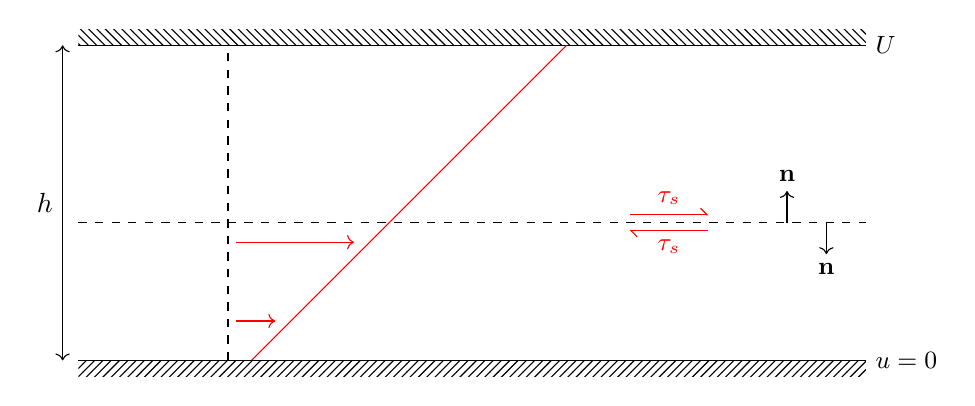
\begin{tikzpicture}
		\draw (-5, -2) -- (5, -2);
		\draw (-5, 2) -- (5, 2);
		\draw[red, ->] (-3, -1.5) -- (-2.5, -1.5);
		\draw[red, ->] (-3, -0.5) -- (-1.5, -0.5);
		\draw[dashed] (-3.1,-2) -- (-3.1,2);
		\draw[dashed] (-5, -0.25) -- (5, -0.25);
		\draw[red] (-2.8,-2) -- (1.2,2);
		\node[right] at (5,-2) {\small $u=0$};
		\node[right] at (5,2) {\small $U$};
		\draw[<->] (-5.2, -2) -- (-5.2, 2);
		\node[left] at (-5.2, 0) {$h$};
		\fill[pattern = north west lines] (-5,2) rectangle +(10,0.2);
		\fill[pattern = north east lines] (-5,-2) rectangle +(10,-0.2);
		\draw[->] (4, -0.25) -- +(0,0.4);
		\node[above] at (4,0.15) {\small $\mathbf{n}$};
		\draw[->] (4.5, -0.25) -- +(0,-0.4);
		\node[below] at (4.5,-0.65) {\small $\mathbf{n}$};
		\draw[-{Straight Barb[left]}, red] (2,-0.15) -- (3,-0.15);
		\node[above, red] at (2.5,-0.15) {\small $\tau_s$};
		\draw[-{Straight Barb[left]}, red] (3,-0.35) -- (2,-0.35);
		\node[below, red] at (2.5,-0.35) {\small $\tau_s$};
	\end{tikzpicture}
\end{figure}

Thus the fluid exerts a shear stress $\mu \frac{\partial u}{\partial y}$ on the bottom plate and $- \mu \frac{\partial u}{\partial y}$ on the top plate.

\subsection{2D Parallel Viscous Flow}
\label{sub:2d_parallel_viscous_flow}

We look at the steady case with $\mathbf{f} = 0$. Since it is steady, there is no acceleration, and hence the forces exerted by the surrounding fluid on the dashed rectangle must balance.

\begin{figure}[h]
	\centering
	\caption{2D Parallel Viscous Flow}
	\label{fig:2d_viscous_flow}
	\begin{tikzpicture}
		\begin{axis}
			[
			xmin = 0,
			xmax = 5,
			axis lines = none
			]
		\addplot [domain = 0.3:5, smooth] {x*x*0.1};
		\end{axis}
		\draw[->] (0,1) -- (1,1);
		\draw[->] (0,2) -- (3,2);
		\draw[->] (0,3) -- (4.5,3);
		\draw[->] (0,4) -- (5.5,4);
		\draw[->] (0,5) -- (6.2,5);
		\draw[dashed] (-3,1.5) rectangle +(10,3);
		\draw[red,->] (5,1.5) -- +(0,-0.4);
		\node[red, below] at (5,1.1) {\small $\mathbf{n}$};
		\draw[red,->] (7,2.5) -- +(0.4,0);
		\node[red,right] at (7.4,2.5) {\small $\mathbf{n}$};
		\draw[red,->] (5,4.5) -- +(0,0.4);
		\node[red, above] at (5,4.9) {\small $\mathbf{n}$};
		\draw[red,->] (-3,3.5) -- +(-0.4,0);
		\node[red, left] at (-3.4,3.5) {\small $\mathbf{n}$};
		\node[right] at (7,4.5) {\small $y + \delta y$};
		\node[right] at (7,1.6) {\small $y$};
		\node[below] at (7,1.5) {\small $x+\delta x$};
		\node[below] at (-3,1.5) {\small $x$};
		\node at (8,3) {\small $p(x+\delta x)$};
		\node at (-3.5,3) {\small $p(x)$};
		\node at (1,0) {\small $u(y)$};
	\end{tikzpicture}
\end{figure}

In the $x$-direction,
\[
p(x) \delta y - p(x + \delta x)\delta y + \mu \frac{\partial u}{\partial y} \biggr|_{y + \delta y} \delta x - \mu \frac{\partial u}{\partial y}|_y \delta x = 0
.\]
Dividing by $\delta x \delta y$, we can take the limit to get
\[
- \frac{\partial p}{\partial x} + \mu \frac{\partial^2 u}{\partial y^2} = 0
.\]
Similarly, in the $y$-direction,
\[
- \frac{\partial p}{\partial y} = 0
.\]

For 2D unsteady parallel viscous flow with $\mathbf{u} = (u(y, t), 0, 0)$ and body force $\mathbf{f} = (f_x, f_y, 0)$, we get
\begin{align*}
	\rho \frac{\partial u}{\partial t} &= - \frac{\partial p}{\partial x} + \mu \frac{\partial^2 u}{\partial y^2} + f_x, \\
	0 &= - \frac{\partial p}{\partial y} + f_y.
\end{align*}
Note our independence of $\mathbf{u}$ on $x$ means $\nabla \cdot \mathbf{u} = 0$ 

It has been verified experimentally (down to molecular scales) that at a rigid boundary, viscous fluids satisfy the \emph{no-slip boundary condition}\index{no-slip boundary condition}
\begin{center}
	the tangential component of the fluid velocity must equal that of the boundary.
\end{center}

We can combine this with the mass conserving kinematic boundary condition
\[
\mathbf{u} = \mathbf{U}
.\]

\begin{figure}[h]
	\centering
	\caption{Pois\'{e}uille Flow}
	\label{fig:poiseuille_flow}
	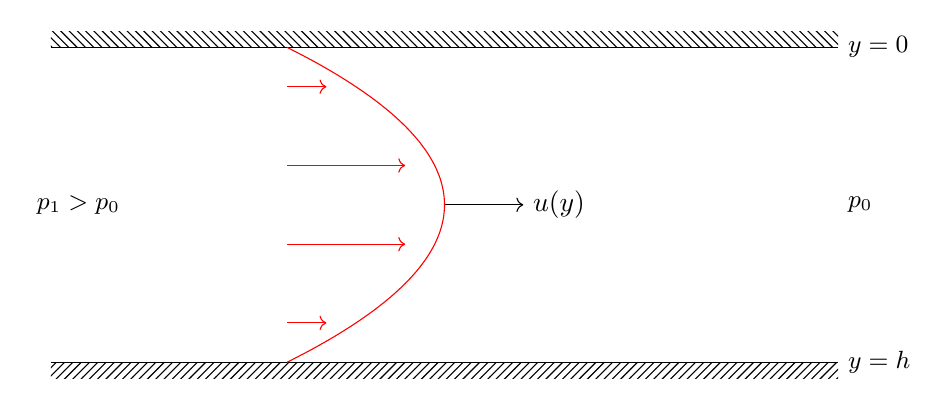
\begin{tikzpicture}
		\draw (-5, -2) -- (5, -2);
		\draw (-5, 2) -- (5, 2);
		\draw[red, ->] (-2, -1.5) -- (-1.5, -1.5);
		\draw[red, ->] (-2, -0.5) -- (-0.5, -0.5);
		\draw[red, ->] (-2, 0.5) -- (-0.5, 0.5);
		\draw[red, ->] (-2, 1.5) -- (-1.5, 1.5);
		\draw[->] (0, 0) -- (1, 0);
		\node[right] at (1, 0) {$u(y)$};
		\node[right] at (5,-2) {\small $y = h$};
		\node[right] at (5,2) {\small $y = 0$};
		\node[left] at (-4, 0) {\small $p_1 > p_0$};
		\node[right] at (5, 0) {\small $p_0$};
		\fill[pattern = north west lines] (-5,2) rectangle +(10,0.2);
		\fill[pattern = north east lines] (-5,-2) rectangle +(10,-0.2);
 		\draw[red]   plot[smooth,domain=-2:2] ({-0.5*(\x)^2}, \x);
	\end{tikzpicture}
\end{figure}

\begin{exbox}[Pois\'{e}uille Flow]
	Consider steady flow in a channel driven by a pressure gradient. We know $\frac{\partial p}{\partial y} = 0$, so $p = p(x)$. As it is steady,
	\[
	\mu \frac{\partial^2 u}{\partial y^2} = \frac{\diff p}{\diff x} = - G
	,\]
	and by no-slip, $u(0) = u(h) = 0$. Hence we can determine
	\[
	u = \frac{G}{2\mu} y(h - y)
	.\]
	This determines a parabolic flow profile. The flux is
	\[
	q = \int_{0}^{h} u \diff y = \frac{G h^3}{12 \mu}
	.\]
	The overall force balance is
	\[
	G h - \mu \frac{\partial u}{\partial u} \biggr|_{0} + \mu \frac{\partial u}{\partial y} \biggr|_{L} = 0
	.\]
\end{exbox}

\begin{figure}[h]
	\centering
	\caption{Viscous Flow down a Slope}
	\label{fig:viscous_slope}
	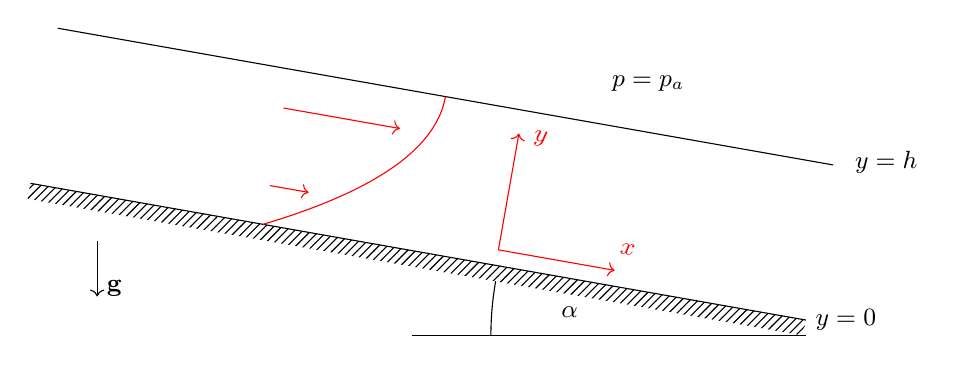
\begin{tikzpicture}
		\draw[rotate around={-10:(5,-2)}] (-5, -2) -- (5, -2);
		\draw[rotate around={-10:(5,-2)}] (-5, 0) -- (5, 0);
		\draw[red, ->, rotate around={-10:(5,-2)}] (-2, -1.5) -- (-1.5, -1.5);
		\draw[red, ->, rotate around={-10:(5,-2)}] (-2, -0.5) -- (-0.5, -0.5);
		\draw[red, ->, rotate around={-10:(5,-2)}] (1, -1.8) -- (2.5,-1.8);
		\node[red, right, rotate around={-10:(5,-2)}] at (2.1,-1.9) {\small $x$};
		\draw[red, ->, rotate around={-10:(5,-2)}] (1, -1.8) -- (1,-0.3);
		\node[red, right, rotate around={-10:(5,-2)}] at (1,-0.5) {\small $y$};
 		\draw[red, rotate around={-10:(5,-2)}]  plot[smooth,domain=-2:0] ({-0.5*(\x)^2}, \x);
%		\node[right] at (5,-2) {\small $y = h$};
%		\node[right] at (5,2) {\small $y = 0$};
		\fill[pattern = north east lines, rotate around={-10:(5,-2)}] (-5,-2) rectangle +(10,-0.2);
		\node[right] at (5, -2) {\small $y = 0$};
		\node[right] at (5.5,0) {\small $y = h$};
		\draw (0,-2.2) -- (5,-2.2);
		\draw (5,-2.2) + (170:4) arc (170:180:4);
		\node at (2,-1.9) {\small $\alpha$};
		\node at (3,1) {\small $p = p_a$};
		\draw[->] (-4,-1) -- (-4, -1.7);
		\node[right] at (-4,-1.6) {\small $\mathbf{g}$};
	\end{tikzpicture}
\end{figure}

\begin{exbox}
	We consider viscous flow down a slope, driven by gravity. Assume that $p_{\mathrm{air}}$ is uniform. Then the shear stress exerted by the air is negligible.

	Take coordinates parallel and perpendicular to the plane. Then the force is $\mathbf{f} = (\rho g \sin \alpha, - \rho g \cos \alpha)$. For the perpendicular force,
	\[
	\frac{\partial p}{\partial y} = \rho g \cos \alpha,
	\]
	which when combined with $p = p_{a}$ at $y = h$ gives
	\[
	p = p_a + \rho g \cos \alpha (h - y)
	,\]
	hence $\frac{\partial p}{\partial h} = 0$. Now the parallel force gives
	\[
	\mu \frac{\partial^2 u}{\partial y^2} = - \rho g \sin \alpha
	.\]
	Then taking $u(0) = 0$ due to no-slip and $\mu \frac{\partial u}{\partial y} |_h = 0$ as there is no shear stress, we get
	\[
	u = \frac{\rho g \sin \alpha}{2 \mu} y(2h - y)
	.\]
\end{exbox}

%Lecture 8

\subsubsection{Boundary Conditions at an Interface}
\label{subsub:boundary_conditions_at_an_interface}

Consider two fluid in parallel viscous flow:
\begin{figure}[h]
	\centering
	\caption{Fluids in Parallel Viscous Flow}
	\label{fig:parallel_viscous_fluids}
	\begin{tikzpicture}
		\draw (-5, 0) -- (5, 0);
		\node[right] at (5, 0) {\small $y = h$};
		\draw (0,0) -- (3,2);
		\draw (0,0) -- (1,-2);
		\node at (-2, 1) {\small $\mu_1$};
		\node at (-2, -1) {\small $\mu_2$};
		\node at (3, 1) {\small $u_1(y)$};
		\node at (3, -1) {\small $u_2(y)$};
	\end{tikzpicture}
\end{figure}
At $y = h$, the boundary of their interface, by the no-slip condition we have $u_1 = u_2$. Hence,
\begin{align*}
	\mu_1 \frac{\partial u_1}{\partial y} &= \mu_2 \frac{\partial u_2}{\partial y}, & p_1 &= p_2
.\end{align*}
These are the \emph{continuity of stress}\index{continuity of stress} conditions.

\subsection{Unsteady Parallel Viscous Flow and Viscous Diffusion}
\label{sub:unsteady_parallel_viscous_flow_and_viscous_diffusion}

Consider a semi-infinite fluid domain $y > 0$, initially at rest, with no applied pressure gradient and $\mathbf{f} = 0$.

At $t = 0$, the boundary of $(y, 0)$ starts to move with velocity $(U, 0)$.

\begin{figure}[h]
	\centering
	\caption{Impulsively Started Flat Plate}
	\label{fig:impulsive_plate}
	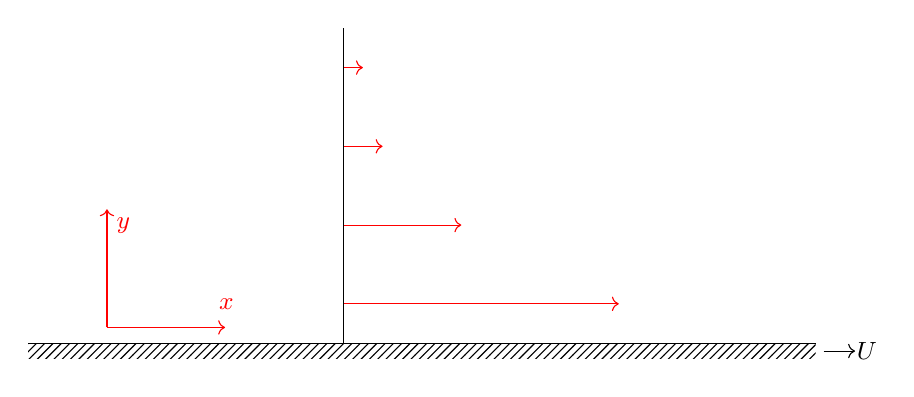
\begin{tikzpicture}
		\draw (-5, -2) -- (5, -2);
		\draw[red, ->] (-1, -1.5) -- (2.5, -1.5);
		\draw[red, ->] (-1, -0.5) -- (0.5, -0.5);
		\draw[red, ->] (-1, 0.5) -- (-0.5, 0.5);
		\draw[red, ->] (-1, 1.5) -- (-0.75, 1.5);
		\draw (-1,-2) -- (-1, 2);
		\draw[->] (5.1,-2.1) -- (5.5,-2.1);
		\node[right] at (5.4,-2.1) {\small $U$};
		\fill[pattern = north east lines] (-5,-2) rectangle +(10,-0.2);
		\draw[red, ->] (-4, -1.8) -- (-2.5,-1.8);
		\node[red, right] at (-2.7,-1.5) {\small $x$};
		\draw[red, ->] (-4, -1.8) -- (-4,-0.3);
		\node[red, right] at (-4,-0.5) {\small $y$};
	\end{tikzpicture}
\end{figure}

Then the change in velocity is subject to the following equations:
\begin{align*}
	\rho \frac{\partial u}{\partial t} = - \frac{\partial p}{\partial x} + \mu \frac{\partial^2 u}{\partial y^2} + f_x,
\end{align*}
as well as initial conditions $u = 0$ at $t = 0$, far-field condition $u = 0$ as $y \to \infty$, and no-slip condition $u = U$ at $y = 0$, $t > 0$.

In the above expression, the first and last term cancel, and we find that the velocity satisfies the \emph{diffusion equation}\index{diffusion equation}
\[
\frac{\partial u}{\partial t} = \nu \frac{\partial^2 u}{\partial y^2}
.\]
Here we are using the kinematic viscosity $\nu = \frac{\mu}{\rho}$, which can be thought of as a measure of diffusivity for momentum (or for viscosity, as we will see later).

From the Methods course, we have many ways of attacking the diffusion equation (e.g. separation of variables, Fourier transforms, Green's functions), which we will use in the example sheet.

Here there is not externally imposed length scale for $y$, since $0 < y < \infty$. However to find a solution we need a length scale! The equation
\[
\frac{\partial u}{\partial t} = \nu \frac{\partial^2 u}{\partial y^2}
\]
suggests that $y \sim (\nu t)^{1/2}$, hence letting $u = U f(\eta)$, where
\[
	\eta = \frac{y}{(\nu t)^{1/2}} \implies \frac{\partial \eta}{\partial t} = -\frac{1}{2} \frac{\partial}{\partial t}
,\]
we can find that $f$ satisfies the equation
\[
- \frac{1}{2} \frac{\eta}{t} U f' = \nu \frac{1}{\nu t} U f''
,\]
which we can then solve as
\begin{align*}
	f'' = -\frac{1}{2} \eta f' &\implies - \frac{1}{2} \eta = \frac{f''}{f'} \\
				   &\implies -\frac{1}{4} \eta^2 = \log f' + \mathrm{constant} \\
				   &\implies f = A + B \int_{\eta}^{\infty} e^{-\frac{1}{4} \eta'^2}\diff \eta'.
\end{align*}
Since $f(\infty) = 0$, we get $A = 0$, and $f(0) = 1$ gives $B = \pi^{-1/2}$, which simplifies to
\[
	u = U \erf \biggl( \frac{y}{2 \sqrt{vt}} \biggr)
.\]
Hence at all times, the shape of the flow is similar, but with growing width as $(vt)^{1/2} \to \infty$.

From dimensional analysis, we could also conclude that $\frac{y}{u t}$ and $\frac{y u}{\nu}$ are dimensionless, but the equations show that these are not relevant. Instead the scaling argument is better!

Below are the kinematic and dynamic viscosities of some fluids.
\begin{center}
	\begin{tabular}{cccc}
		& $\rho$ & $\mu$ & $\nu$ \\
		Water & \qty{1e3}{\kilogram \meter \tothe{-3}} & \qty{1e-3}{\pascal \second} & \qty{1e-6}{\meter \squared \per \second} \\
		Air & \qty{1}{\kilogram \metre \tothe{-3}} & \qty{2 e-5}{\pascal \second} & \qty{2 e-5}{\meter \squared \per \second} \\
		Golden Syrup & \qty{1.4e3}{\kilogram \meter \tothe{-3}} & \qty{200}{\pascal \second} & \qty{0.14}{\meter \squared \per \second}
	\end{tabular}
\end{center}
Since $\nu_{\mathrm{air}} \approx 10 \nu_{\mathrm{water}}$, momentum spreads faster and further in air.

Moreover since the shear stress exerted by a fluid (as in the plate) is
\[
	\tau_s = \mu \frac{\partial u}{\partial y} = - \mu \frac{u}{(vt)^{1/2}}f'(0) = - \frac{\mu U}{\sqrt{\pi \nu t}}
,\]
and we have
\[
	\frac{\mu}{\sqrt{\nu}}\biggr|_{\mathrm{water}} \approx 100 \frac{\mu}{\sqrt{\nu}}\biggr|_{\mathrm{air}}
,\]
water exerts a much bigger stress.

If we add a stationary boundary at $y = h$, then we have two relevant length scales: $h$ and $(\nu t)^{1/2}$.

\begin{figure}[h]
	\centering
	\caption{Started and Steady Plates}
	\label{fig:started_and_steady}
	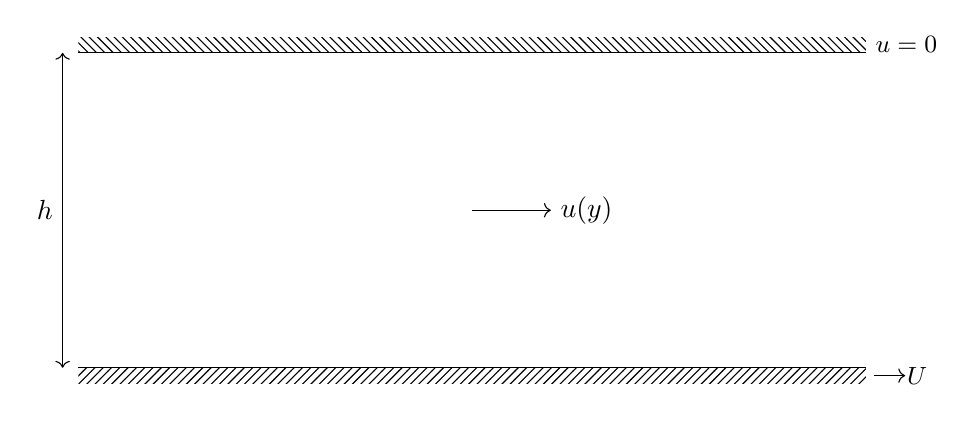
\begin{tikzpicture}
		\draw (-5, -2) -- (5, -2);
		\draw (-5, 2) -- (5, 2);
		\node[right] at (5,2.1) {\small $u=0$};
		\draw[->] (5.1,-2.1) -- (5.5,-2.1);
		\node[right] at (5.4,-2.1) {\small $U$};
		\draw[<->] (-5.2, -2) -- (-5.2, 2);
		\node[left] at (-5.2, 0) {$h$};
		\fill[pattern = north west lines] (-5,2) rectangle +(10,0.2);
		\fill[pattern = north east lines] (-5,-2) rectangle +(10,-0.2);
		\draw[->] (0, 0) -- (1, 0);
		\node[right] at (1, 0) {$u(y)$};
	\end{tikzpicture}
\end{figure}

If we have $h \gg (\nu t)^{1/2}$, then we expect the boundary to have little (exponentially small) effect on the previous solution.

However as $t \to \infty$, we expect to approach steady Couette flow, with a linear profile. Deviations from this steady state decay like $e^{-kt}$, with $k \propto \frac{\nu}{h^2}$, and are small for $\nu t \gg h^2$.

The characteristic timescale is $T = \frac{h^2}{\nu}$ for diffusion across the cell. If $t \ll T$, then the effects of viscosity are confined to the bounding layers with $\delta \sim (vt)^{1/2}$.

If we have a single oscillating boundary, then there is an imposed timescale $\frac{1}{\omega}$ during which velocity variations can diffuse with $\delta \sim (\frac{\nu}{\omega})^{1/2}$.

\begin{figure}[h]
	\centering
	\caption{Oscillating Boundary}
	\label{fig:oscillating}
	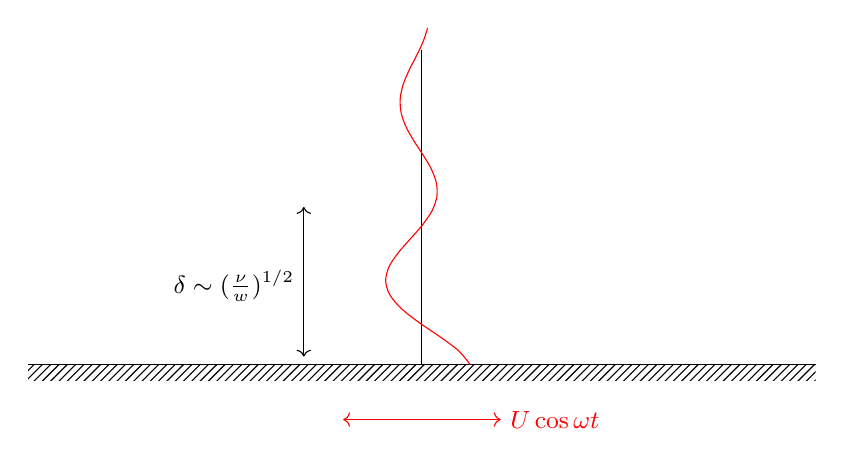
\begin{tikzpicture}
		\draw (-1.5, 0) -- (8.5, 0);
		\draw (3.5,0) -- (3.5, 4);
		\fill[pattern = north east lines] (-1.5,0) rectangle +(10,-0.2);
		\draw[red, <->] (2.5, -0.7) -- (4.5,-0.7);
		\node[red, right] at (4.5, -0.7) {\small $U \cos \omega t$};
		\begin{axis}
			[
			xmin = -5,
			xmax = 5,
			ymin = 0,
			ymax = 4,
			axis lines = none
			]
		\addplot [domain = 0:3, smooth, red] (cos(4 * deg(x)) * (x+1)^(-1), x);
		\end{axis}
		\draw[<->] (2, 0.1) -- (2,2);
		\node[left] at (2, 1) {\small $\delta \sim (\frac{\nu}{w})^{1/2}$};
	\end{tikzpicture}
\end{figure}

%Lecture 9

Adding a stationary boundary to the oscillating boundary gives two timescales $\frac{\nu}{h^2}$ and $\frac{1}{\omega}$, and two length scales $(\frac{\nu}{\omega})^{1/2}$ and $h$. Hence we can determine a dimensionless parameter
\[
S = \frac{\omega h^2}{\nu}
,\]
which is the \emph{Stokes number}\index{Stokes number}.

$S \gg 1$ looks like example the oscillating boundary with $\delta \approx (\nu/w)^{1/2} \ll h$. $S \ll 1$ looks like Couette flow (linear profile) with amplitude $U(t)$.

These examples illustrate that the inviscid solution ($\nu \approx 0$, so $u = 0$ and slipping at boundary) is not uniformly the same as the limit of a ``small'' viscosity (where smallness means $\nu \ll \frac{h^2}{t}$ or $\omega h^2$), but the viscous effects are only felt in the boundary layers $\delta \ll h$.

\subsection{The Navier-Stokes Equation}
\label{sub:the_navier_stokes_equation}

In part II, it is shown that
\[
	\bm{\tau}(\mathbf{x}, t ; \mathbf{n}) = - p \mathbf{n} + \mu[(\mathbf{n} \cdot \nabla) \mathbf{u} + (\nabla \mathbf{u}) \cdot \mathbf{n}],
\]
and hence the flow satisfies the \emph{Navier-Stokes equation}\index{Navier-Stokes equation}
\[
\rho \frac{D \mathbf{u}}{Dt} = - \nabla p + \mu \nabla^2 \mathbf{u} + \mathbf{f}
,\]
and $\nabla \cdot \mathbf{u} = 0$. This reduces to the Euler equation if $\mu = 0$, and is parallel to the viscous flow equations if $\mathbf{u} = (u(y,t),0,0)$.

\subsubsection{The Reynolds Number}
\label{subsub:the_reynolds_number}

Suppose a flow has a characteristic lengthscale $L$ and velocity scale $U$ 

%E.g. picture

Assume the characteristic timescale $T$ is $\frac{L}{U}$ (or the flow is steady) and let the characteristic scale of the pressure differences be denoted by $P$.

We can estimate the scale of the terms in the Navier-Stokes equation as
\begin{align*}
	\frac{\partial \mathbf{u}}{\partial t} + \mathbf{u} \cdot \nabla \mathbf{u} &= - \frac{1}{\rho} \nabla p + \nu \nabla^2 \mathbf{u} \\
	\frac{U}{L/U}\qquad  \frac{U^2}{L} &\qquad \frac{p}{\rho L} \qquad  \frac{\nu U}{L^2} \\
	1\quad :\quad 1\quad  &: \quad \frac{p}{\rho U^2}\: : \: \frac{\nu}{LU} \equiv \frac{1}{R_e}
\end{align*}
The \emph{Reynolds number} $\Rey = \frac{UL}{\nu}$ is a dimensionless parameter describing the relative importance of inertia and viscosity:
\[
\frac{p D \mathbf{u}/Dt}{\mu \nabla^2 \mathbf{u}} \sim \Rey
.\]
\begin{itemize}
	\item If $\Rey \ll 1$, then we expect
		\[
		\rho \frac{D \mathbf{u}}{Dt} \ll \mu \nabla^2 \mathbf{u}
		,\]
		so inertia is negligible, and we can approximate the Navier-Stokes equation by the Stokes equations\index{Stokes equations}
		\[
		0 = - \nabla p + \mu \nabla^2 \mathbf{u} + \mathbf{f}, \qquad \nabla \cdot \mathbf{u} = 0.
		\]
		Scaling for pressure is $p \sim \frac{\mu U}{L}$, like the viscous stress.
	\item If $\Rey \gg 1$, we expect
		\[
		\mu \nabla^2 \mathbf{u} \ll \rho \frac{D \mathbf{u}}{Dt}
		,\]
		and hence viscosity is negligible (except perhaps in thin boundary layers at rigid boundaries). We can approximate the Navier-Stokes equation by the Euler equation
		\[
		\rho \frac{D \mathbf{u}}{Dt} = - \nabla p + \mathbf{f}
		,\]
		outside the boundary layer. Pressure scaling is $p \sim \rho U^2$, like Bernoulli.
\end{itemize}

For large Reynolds numbers, and on timescale $L/U$, viscous diffusion affects the velocity over a distance
\[
\delta \sim \biggl( v \frac{L}{U} \biggr)^{1/2}, \qquad \frac{\delta}{L} \sim \biggl( \frac{v}{LU}\biggr)^{1/2} = \frac{1}{\Rey^{1/2}}
.\]

\subsection{Stagnation Point Flow}
\label{sub:stagnation_point_flow}

\begin{figure}[h]
	\centering
	\caption{Stagnation Point}
	\label{fig:stagnation_point}
	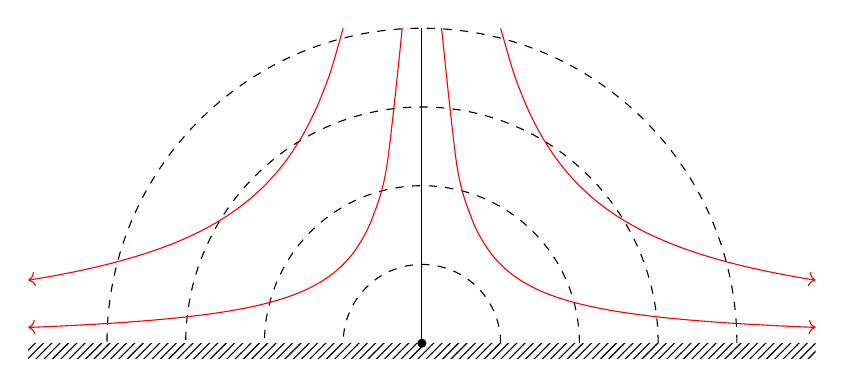
\begin{tikzpicture}
		\fill[pattern = north east lines] (-5,0) rectangle +(10,-0.2);
		\draw (0, 0) -- +(0,4);
		\draw[dashed] (0:1) arc (0:180:1);
		\draw[dashed] (0:2) arc (0:180:2);
		\draw[dashed] (0:3) arc (0:180:3);
		\draw[dashed] (0:4) arc (0:180:4);
		\draw[red, ->]   plot[smooth,domain=0.25:5] (\x, {1/(\x)});
		\draw[red, ->]   plot[smooth,domain=0.25:5] (-1 * \x, {1/(\x)});
		\draw[red, ->]   plot[smooth,domain=1:5] (\x, {4/(\x)});
		\draw[red, ->]   plot[smooth,domain=1:5] (-1 * \x, {4/(\x)});
		\draw[fill] (0,0) circle (0.05);
	\end{tikzpicture}
\end{figure}

Consider the 2D inviscid incompressible flow with $\mathbf{u} = (Ex, -Ey)$ for $y > 0$. Then $\psi = Exy$, and by Bernoulli,
\[
p = p_0 - \frac{1}{2} \rho E^2(x^2 + y^2)
.\]
This solves $\rho (\mathbf{u} \cdot \nabla)\mathbf{u} = - \nabla p$, with $v = 0$ on $y = 0$.

This also satisfies the Navier-Stokes equations, but not the viscous no-slip boundary condition because $u = 0$ if $y = 0$ is a rigid boundary. Fortunately, we can find an exact solution. Guessing
\[
\psi = Ex f(y) \implies \mathbf{u} = (E_x f', -Ef)
,\]
we want $f(0) = f'(0) = 0$ and $f(y) \approx y$ as $y \to \infty$. Substituting into
\[
	(\mathbf{u} \cdot \nabla)\mathbf{u} = - \frac{1}{\rho} \nabla p + \nu \nabla^2 \mathbf{u}
,\]
the $x$-component gives
\begin{align*}
	\biggl(E_x f' \frac{\partial}{\partial x} - E f \frac{\partial}{\partial y}\biggr) E_x f' &= - \frac{1}{\rho} \frac{\partial p}{\partial x} + \nu \biggl( \frac{\partial^2}{\partial x^2} + \frac{\partial^2}{\partial y^2} \biggr) (E_x f') \\
	\implies E^2 x(f'^2 - ff'') &= - \frac{1}{\rho} \frac{\partial p}{\partial u} + \nu E_x f'''.
\end{align*}
Similarly, the $y$-component gives
\[
	E^2 f' f = - \frac{1}{\rho} \frac{\partial p}{\partial y} - \nu E f''
.\]
Taking the $x$ derivative of this equation gives
\[
\frac{\partial^2 p}{\partial x \partial y} = 0 \implies p = X(x) + Y(y)
.\]
Then from the first equation,
\[
\frac{\partial p}{\partial x} \propto x, \qquad f' \to 1 \implies X(x) = p_0 - \frac{1}{2} \rho E^2 x^2
.\]
Hence
\[
f'^2 - ff'' = 1 + \frac{\nu}{E} f'''
.\]
Rescaling, $f(y) = \delta F(\eta)$, where $\eta = \frac{y}{\delta}$ and $\delta = (\frac{\nu}{E})^{1/2}$. So,
\[
	F''' = F'^2 - FF'' - 1, \qquad F(0) = F'(0) = 0, \qquad F'(1) \overset{y \to \infty}{\to} 1
.\]
We can solve this numerically.

\newpage

\printindex

\end{document}
